\documentclass[a4paper]{article}

%------------------------------------------------------------
\usepackage[a4paper, total={6in, 9in}]{geometry}
\usepackage{amsmath, amssymb}
\usepackage{booktabs}
\usepackage{caption}
\usepackage{enumitem}
\usepackage{graphicx}
\usepackage{float}
\usepackage{inconsolata}
\usepackage{listings}
\usepackage{mathtools}
\usepackage{pstricks-add}
\usepackage{siunitx}
\usepackage[most]{tcolorbox}
\usepackage{tikz, pgfplots}
\usepackage{epstopdf} %converting to PDF
\usepackage{hyperref}
\usepackage{xfrac}

\usetikzlibrary{shapes.geometric}
\usetikzlibrary{arrows}
\usetikzlibrary{calc}

%------------------------------------------------------------
\graphicspath{{./fig/}}
\pgfplotsset{compat=1.13}
%------------------------------------------------------------
\setlength{\parindent}{0in}

\lstdefinestyle{C++}{
	language=C++,
	basicstyle=\ttfamily,
	keywordstyle=\color{blue}\ttfamily,
	stringstyle=\color{red}\ttfamily,
	commentstyle=\color{green}\ttfamily,
	morecomment=[l][\color{magenta}]{\#},
	showstringspaces=false
}

%------------------------------------------------------------
\newtcblisting[auto counter]{sexylisting}[2][]{sharp corners, 
    fonttitle=\bfseries, colframe=gray, listing only, 
    listing options={basicstyle=\ttfamily,language=C++}, 
    title=Listing \thetcbcounter: #2, #1}

%------------------------------------------------------------
\lstset{language=C++,
        basicstyle=\ttfamily,
        keywordstyle=\color{blue}\ttfamily,
        stringstyle=\color{red}\ttfamily,
        commentstyle=\color{green}\ttfamily,
        morecomment=[l][\color{magenta}]{\#},
        showstringspaces=false
}
%------------------------------------------------------------
\tikzstyle{block} = [draw, fill=blue!20, rectangle, 
    minimum height=3em, minimum width=3em]
\tikzstyle{sum} = [draw, fill=blue!20, circle, node distance=1cm]
\tikzstyle{input} = [coordinate]
\tikzstyle{output} = [coordinate]
\tikzstyle{pinstyle} = [pin edge={to-,thin,black}]

%------------------------------------------------------------
\newlength{\arrow}
\settowidth{\arrow}{\scriptsize$1000$}

\newcommand*{\myrightarrow}[1]{\xrightarrow{\mathmakebox[\arrow]{#1}}}

\newcommand{\uvec}[1]{\boldsymbol{\hat{\textbf{#1}}}}

%------------------------------------------------------------

\begin{document}
\title{ENG252 Dynamics: Project}
\author{Shane Reynolds}
\maketitle

\section{Introduction and Scope}

\section{Design}

\begin{figure}[h]
	\centering
	\begin{minipage}{0.55\textwidth}
		\centering
		\frame{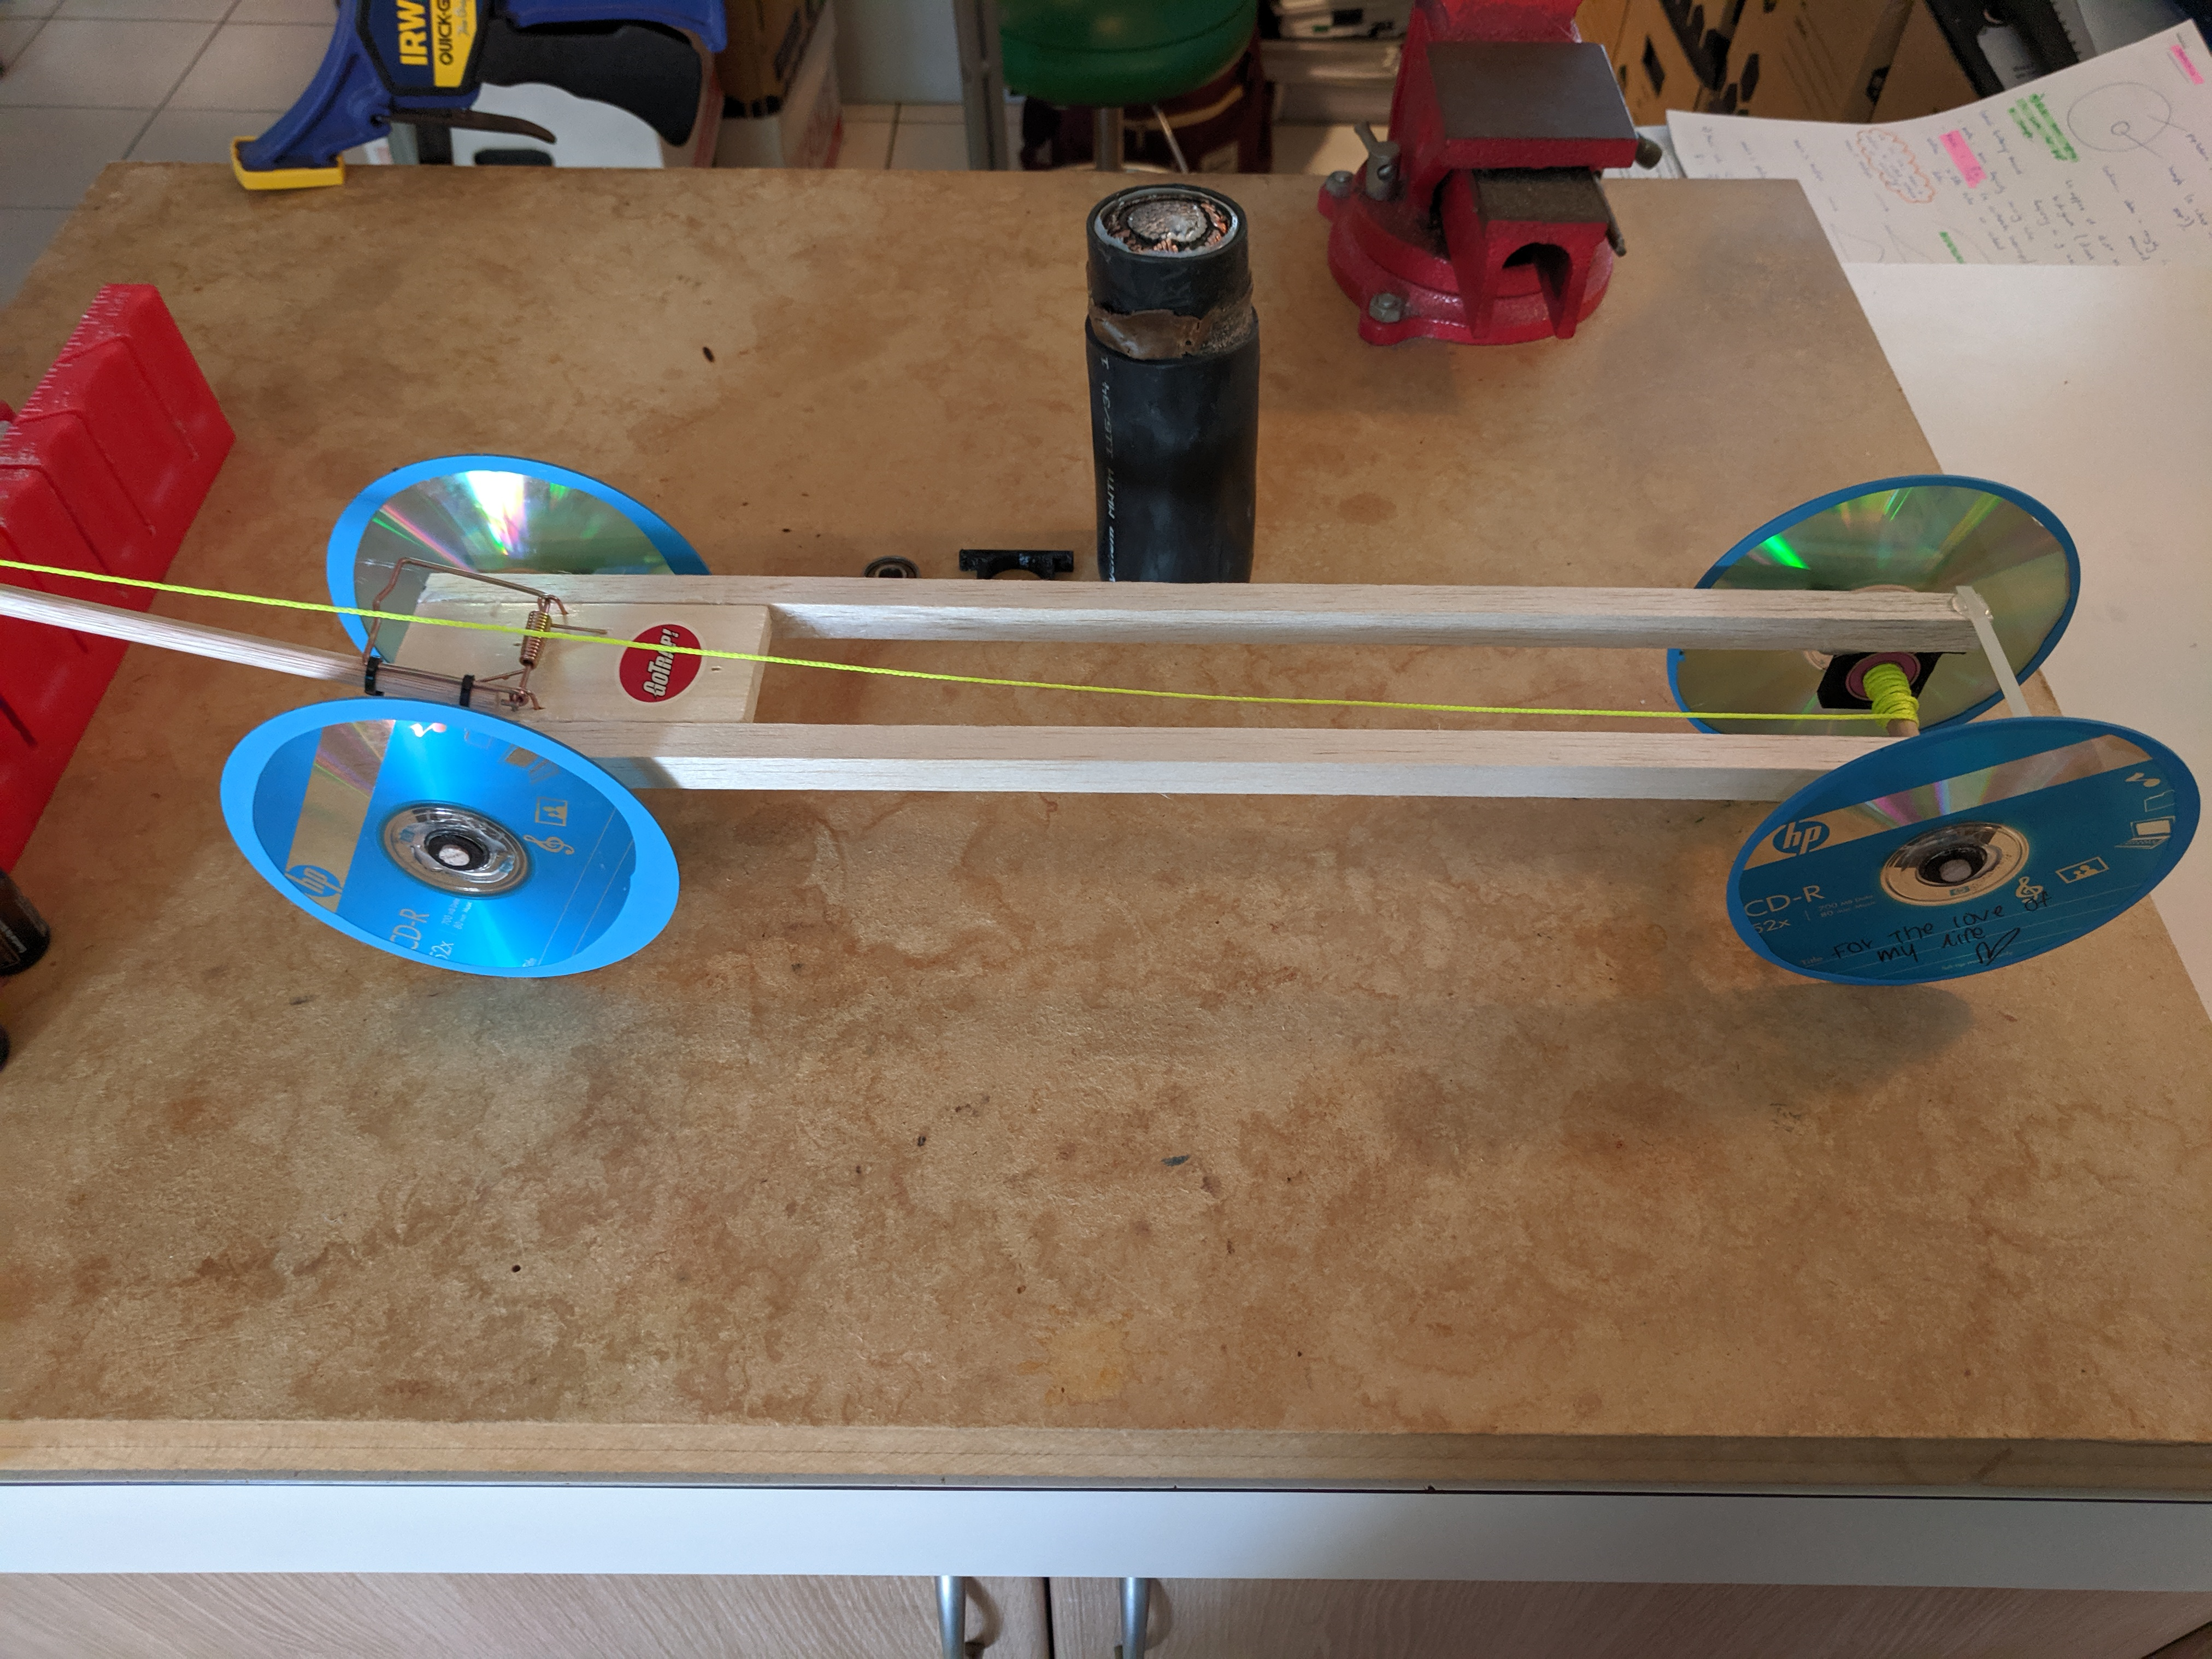
\includegraphics[height=6cm]{car}}
		\caption{Vehicle material selection predominately focused on limiting the vehicle mass. Where possible existing structures, such as Compact discs, were used to reduce manufacturing effort.}
	\end{minipage}
	\hspace{0.5cm}
	\begin{minipage}{0.35\textwidth}
		\centering
		\captionof{table}{Key vehicle characteristics.}
		\begin{tabular}{lrc}
			\toprule
			Measurement & Value & Unit \\
			\midrule
			Chassis Length & & \\
			Chassis Width & & \\
			Chassis Height & & \\
			Mass & 0.180 & $\si{\kilogram}$ \\
			\bottomrule
		\end{tabular}
	\end{minipage}
	
\end{figure}

\begin{figure}[h]
	\centering
	\begin{minipage}[t]{0.45\textwidth}
		\centering
		\frame{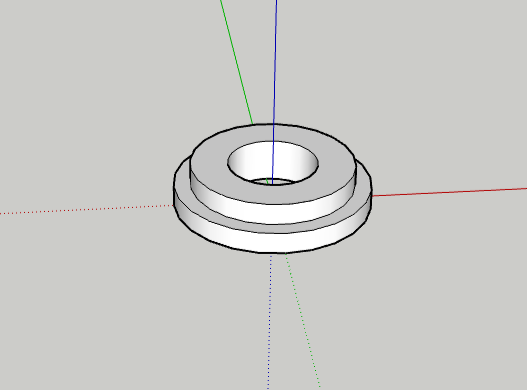
\includegraphics[height=5cm]{cd_mount_design}}
		\caption{Small plastic mounts designed to securely fix the shaft to the Compact Disc wheel at the centre of mass.}
	\end{minipage}
	\hspace{1cm}
	\begin{minipage}[t]{0.45\textwidth}
		\centering
		\frame{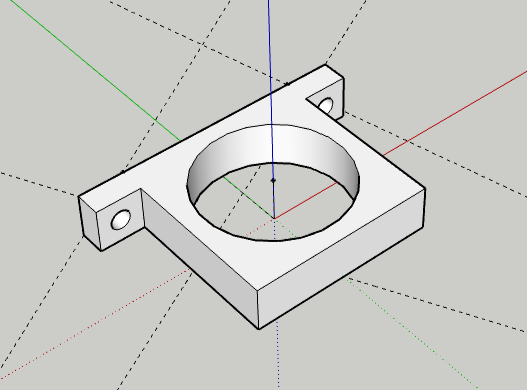
\includegraphics[height=5cm]{bearing_mount_design}}
		\caption{Small plastic mounts designed to house the bearings and attach them securely to the vehicle chassis.}
	\end{minipage}
\end{figure}

\begin{figure}[h]
	\centering
	\begin{minipage}[t]{0.45\textwidth}
		\centering
		\begin{tabular}{p{3.5cm}rc}
			\toprule
			Measurement & Value & Unit \\
			\midrule
			Length & 0.450 & $\si{\meter}$ \\
			Width & 0.010 & $\si{\meter}$  \\
			Mass & 0.006 & $\si{\kilogram}$ \\
			\bottomrule
		\end{tabular}
		
		\vspace{0.5cm}
		
		\frame{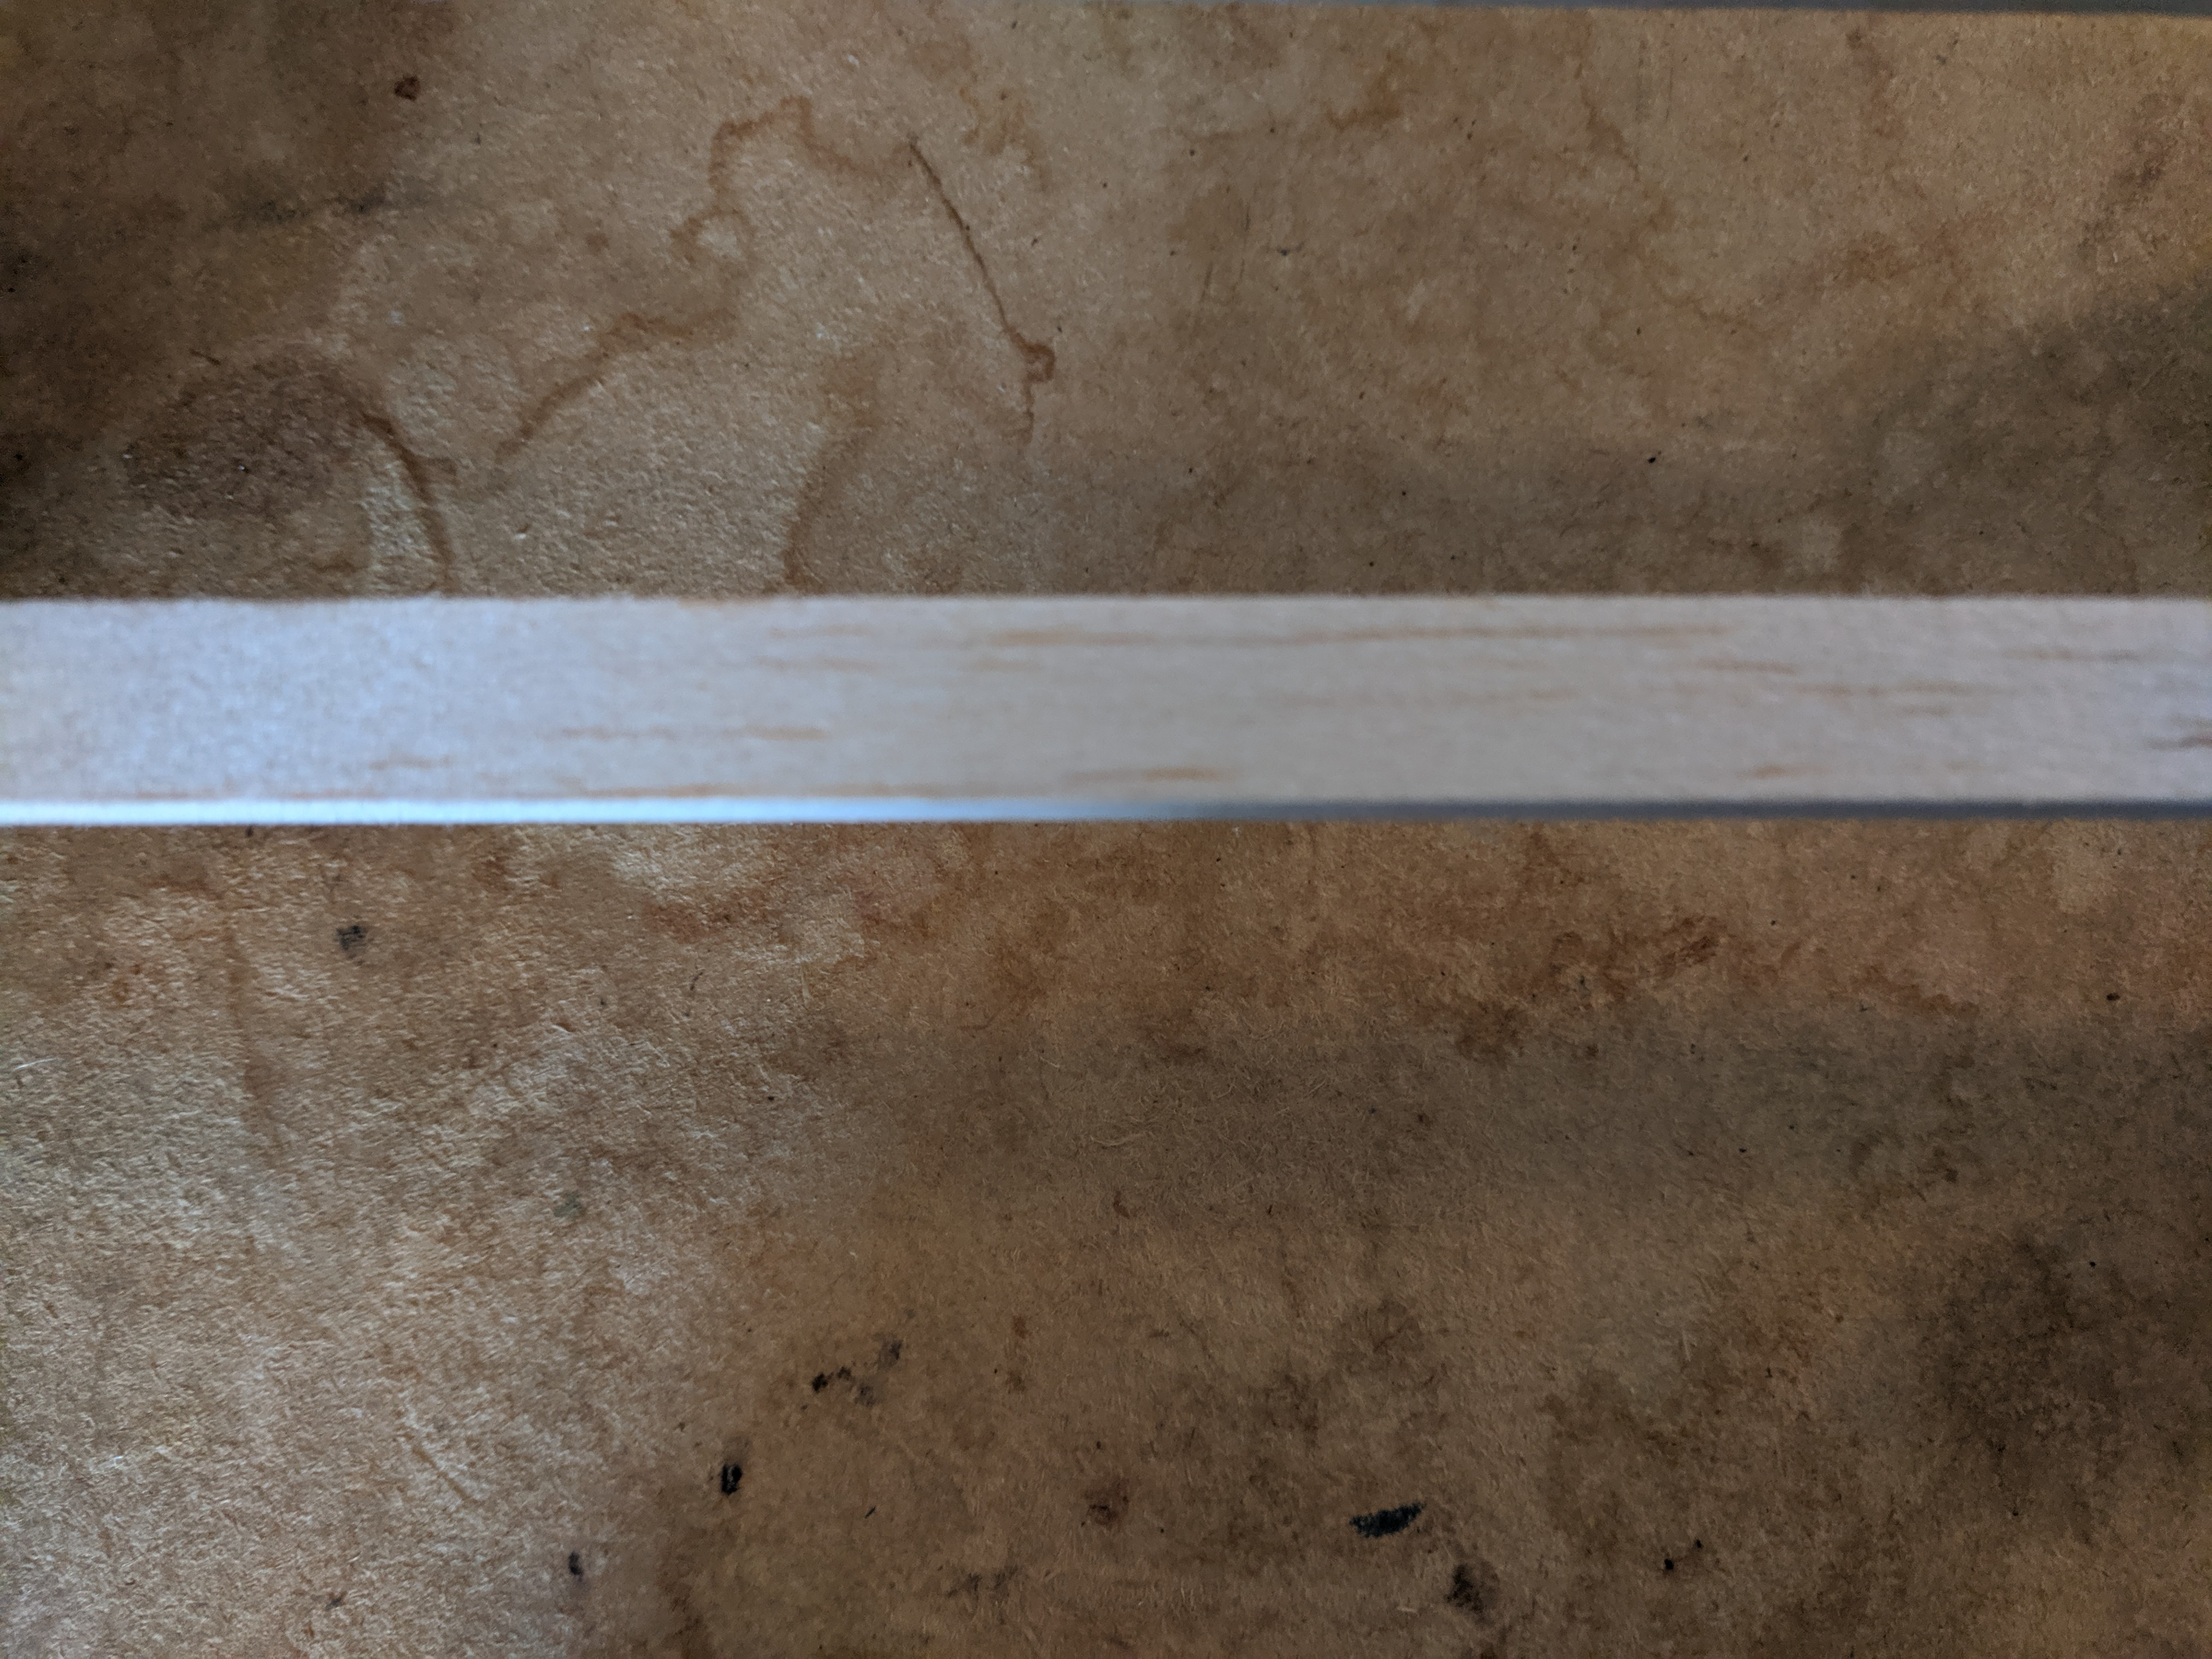
\includegraphics[height=5cm]{balsa_frame}}
		\caption{Balsa wood section used for the frame. Two lengths were used.}
	\end{minipage}
	\hspace{1cm}
	\begin{minipage}[t]{0.45\textwidth}
		\centering
		\begin{tabular}{p{3.5cm}rc}
			\toprule
			Measurement & Value & Unit \\
			\midrule
			Diameter & 0.022 & $\si{\meter}$ \\
			Mass & 0.009 & $\si{\kilogram}$ \\
			 & \\
			\bottomrule
		\end{tabular}
		
		\vspace{0.5cm}
		
		\frame{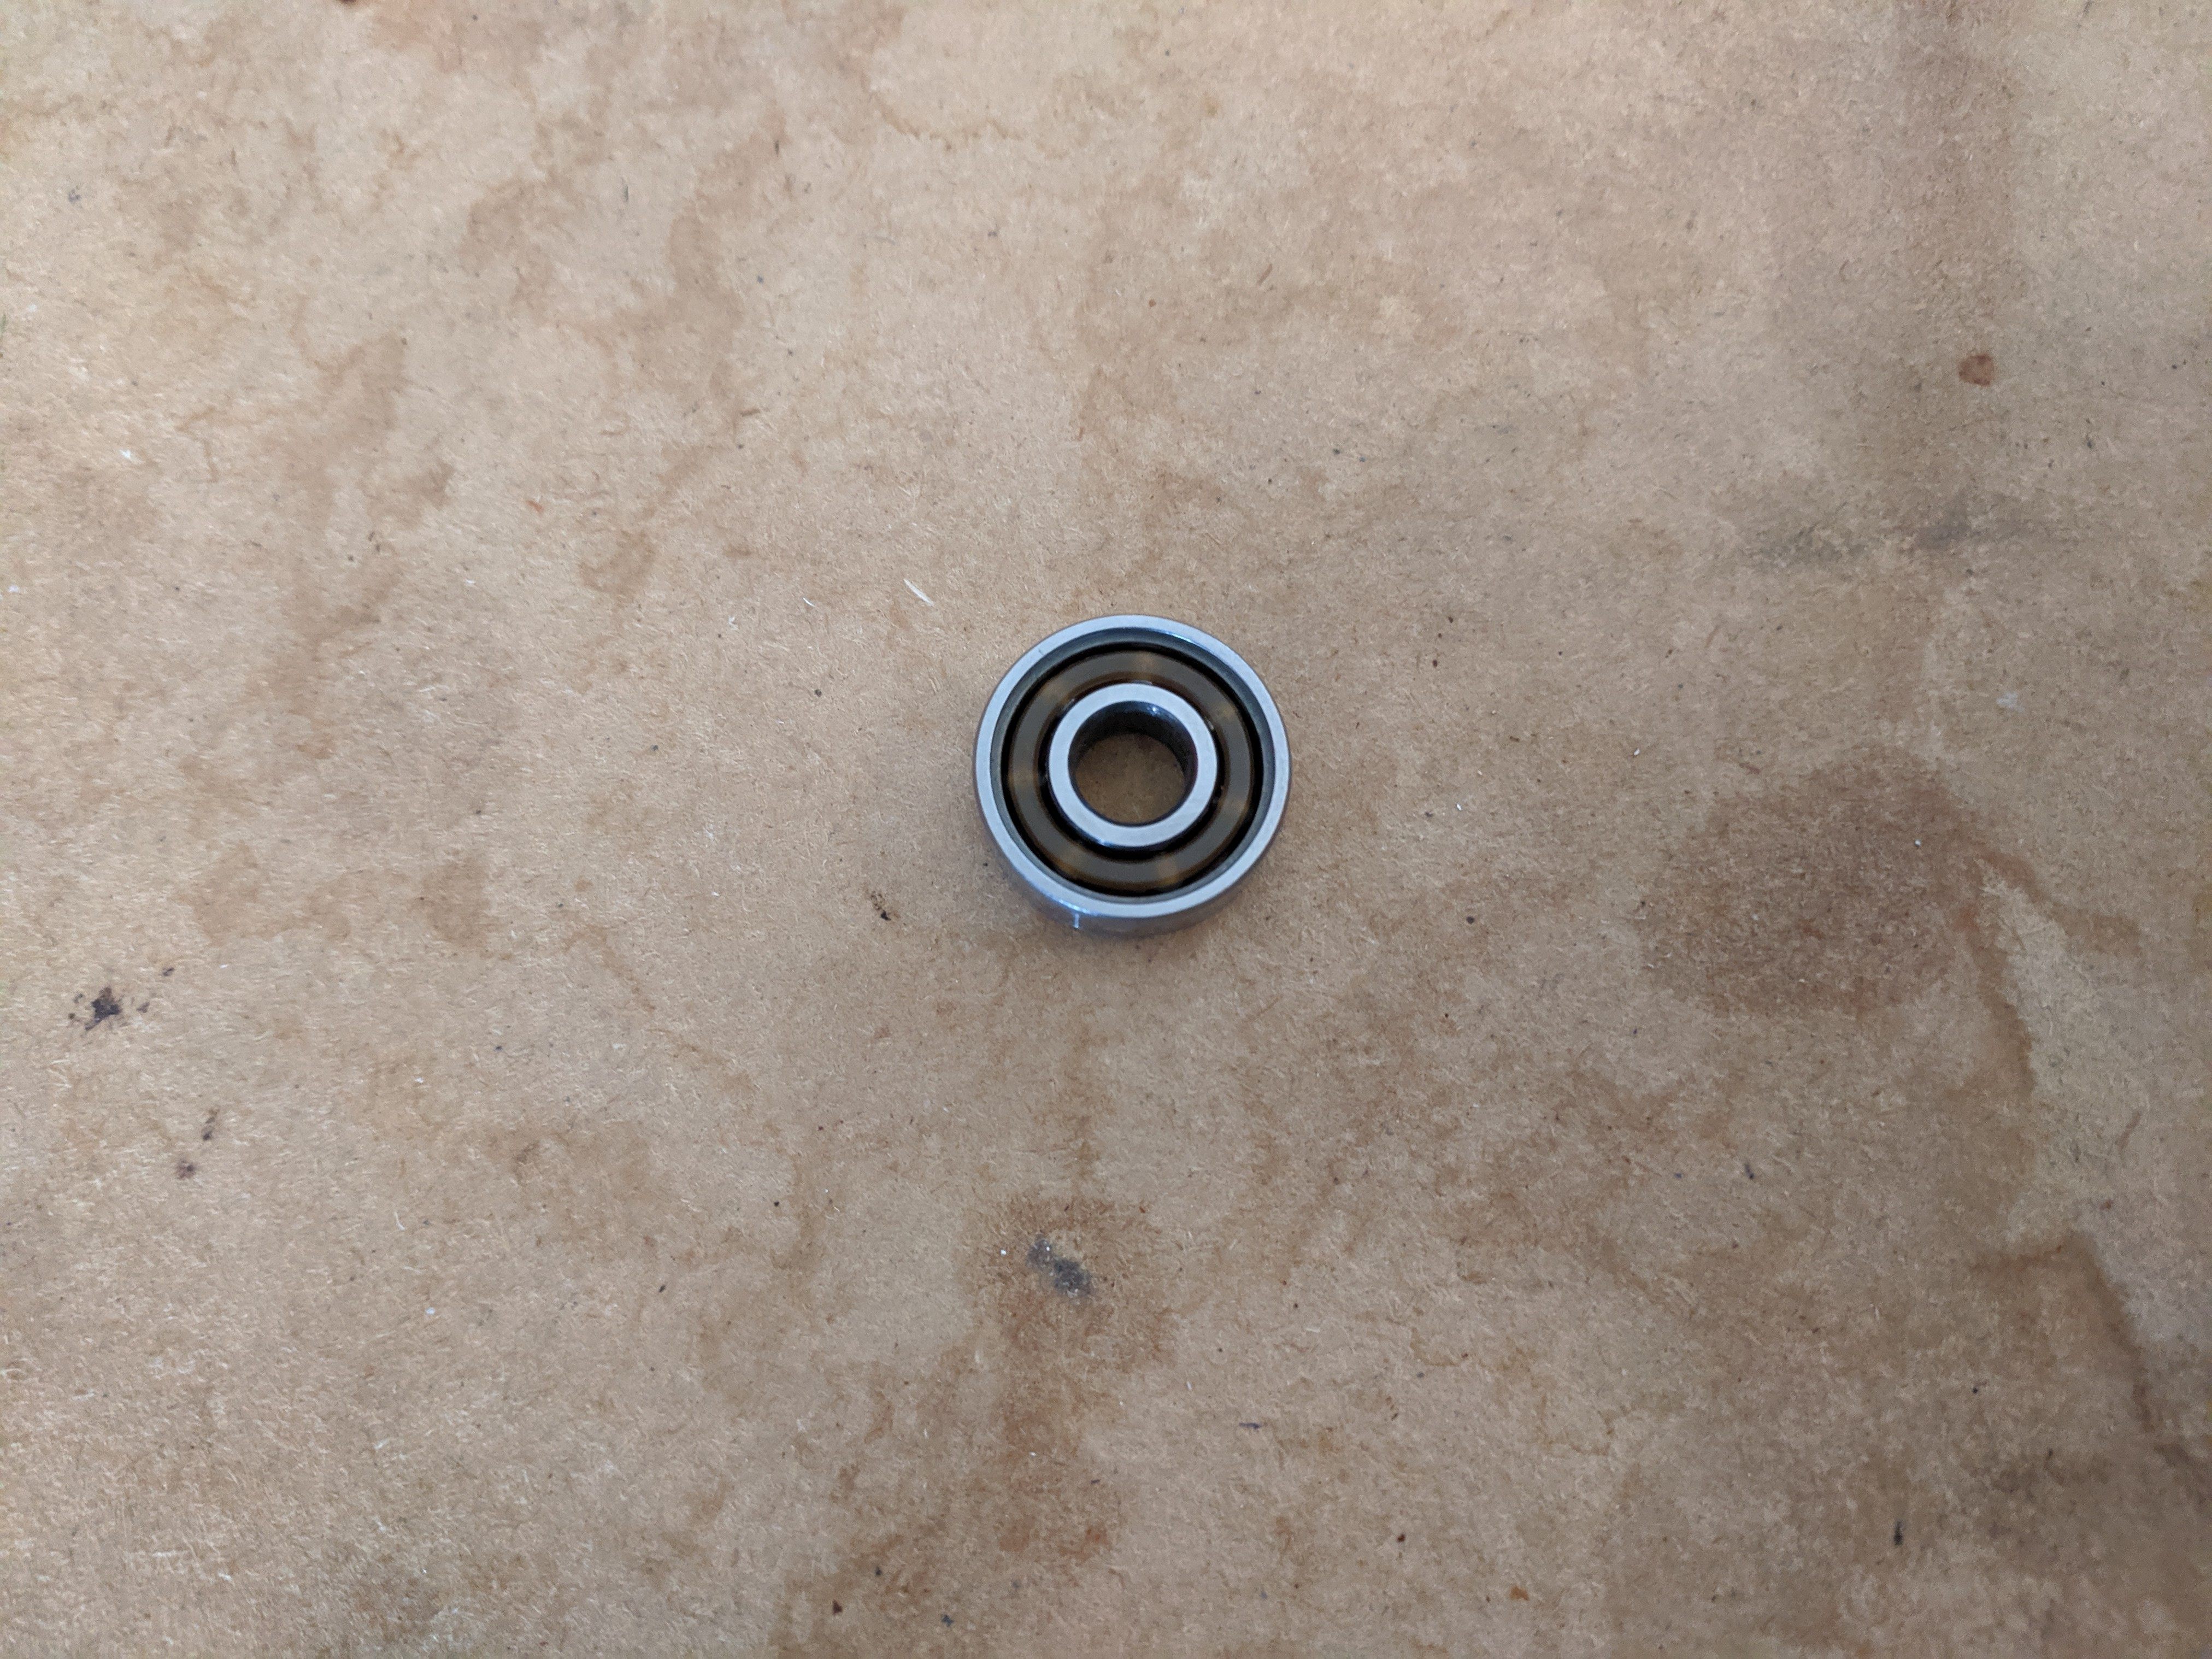
\includegraphics[height=5cm]{bearing}}
		\caption{Bearings used to reduce friction between shafts and frame.}
	\end{minipage}
\end{figure}


\begin{figure}[h]
	\centering
	\begin{minipage}[t]{0.45\textwidth}
		\centering
		
		\begin{tabular}{p{3.5cm}rc}
			\toprule
			Measurement & Value & Unit \\
			\midrule
			Length & 0.028 & $\si{\meter}$ \\
			Width & 0.028 & $\si{\meter}$ \\
			Mass & 0.002 & $\si{\kilogram}$ \\
			\bottomrule
		\end{tabular}
		
		\vspace{0.5cm}
		
		\frame{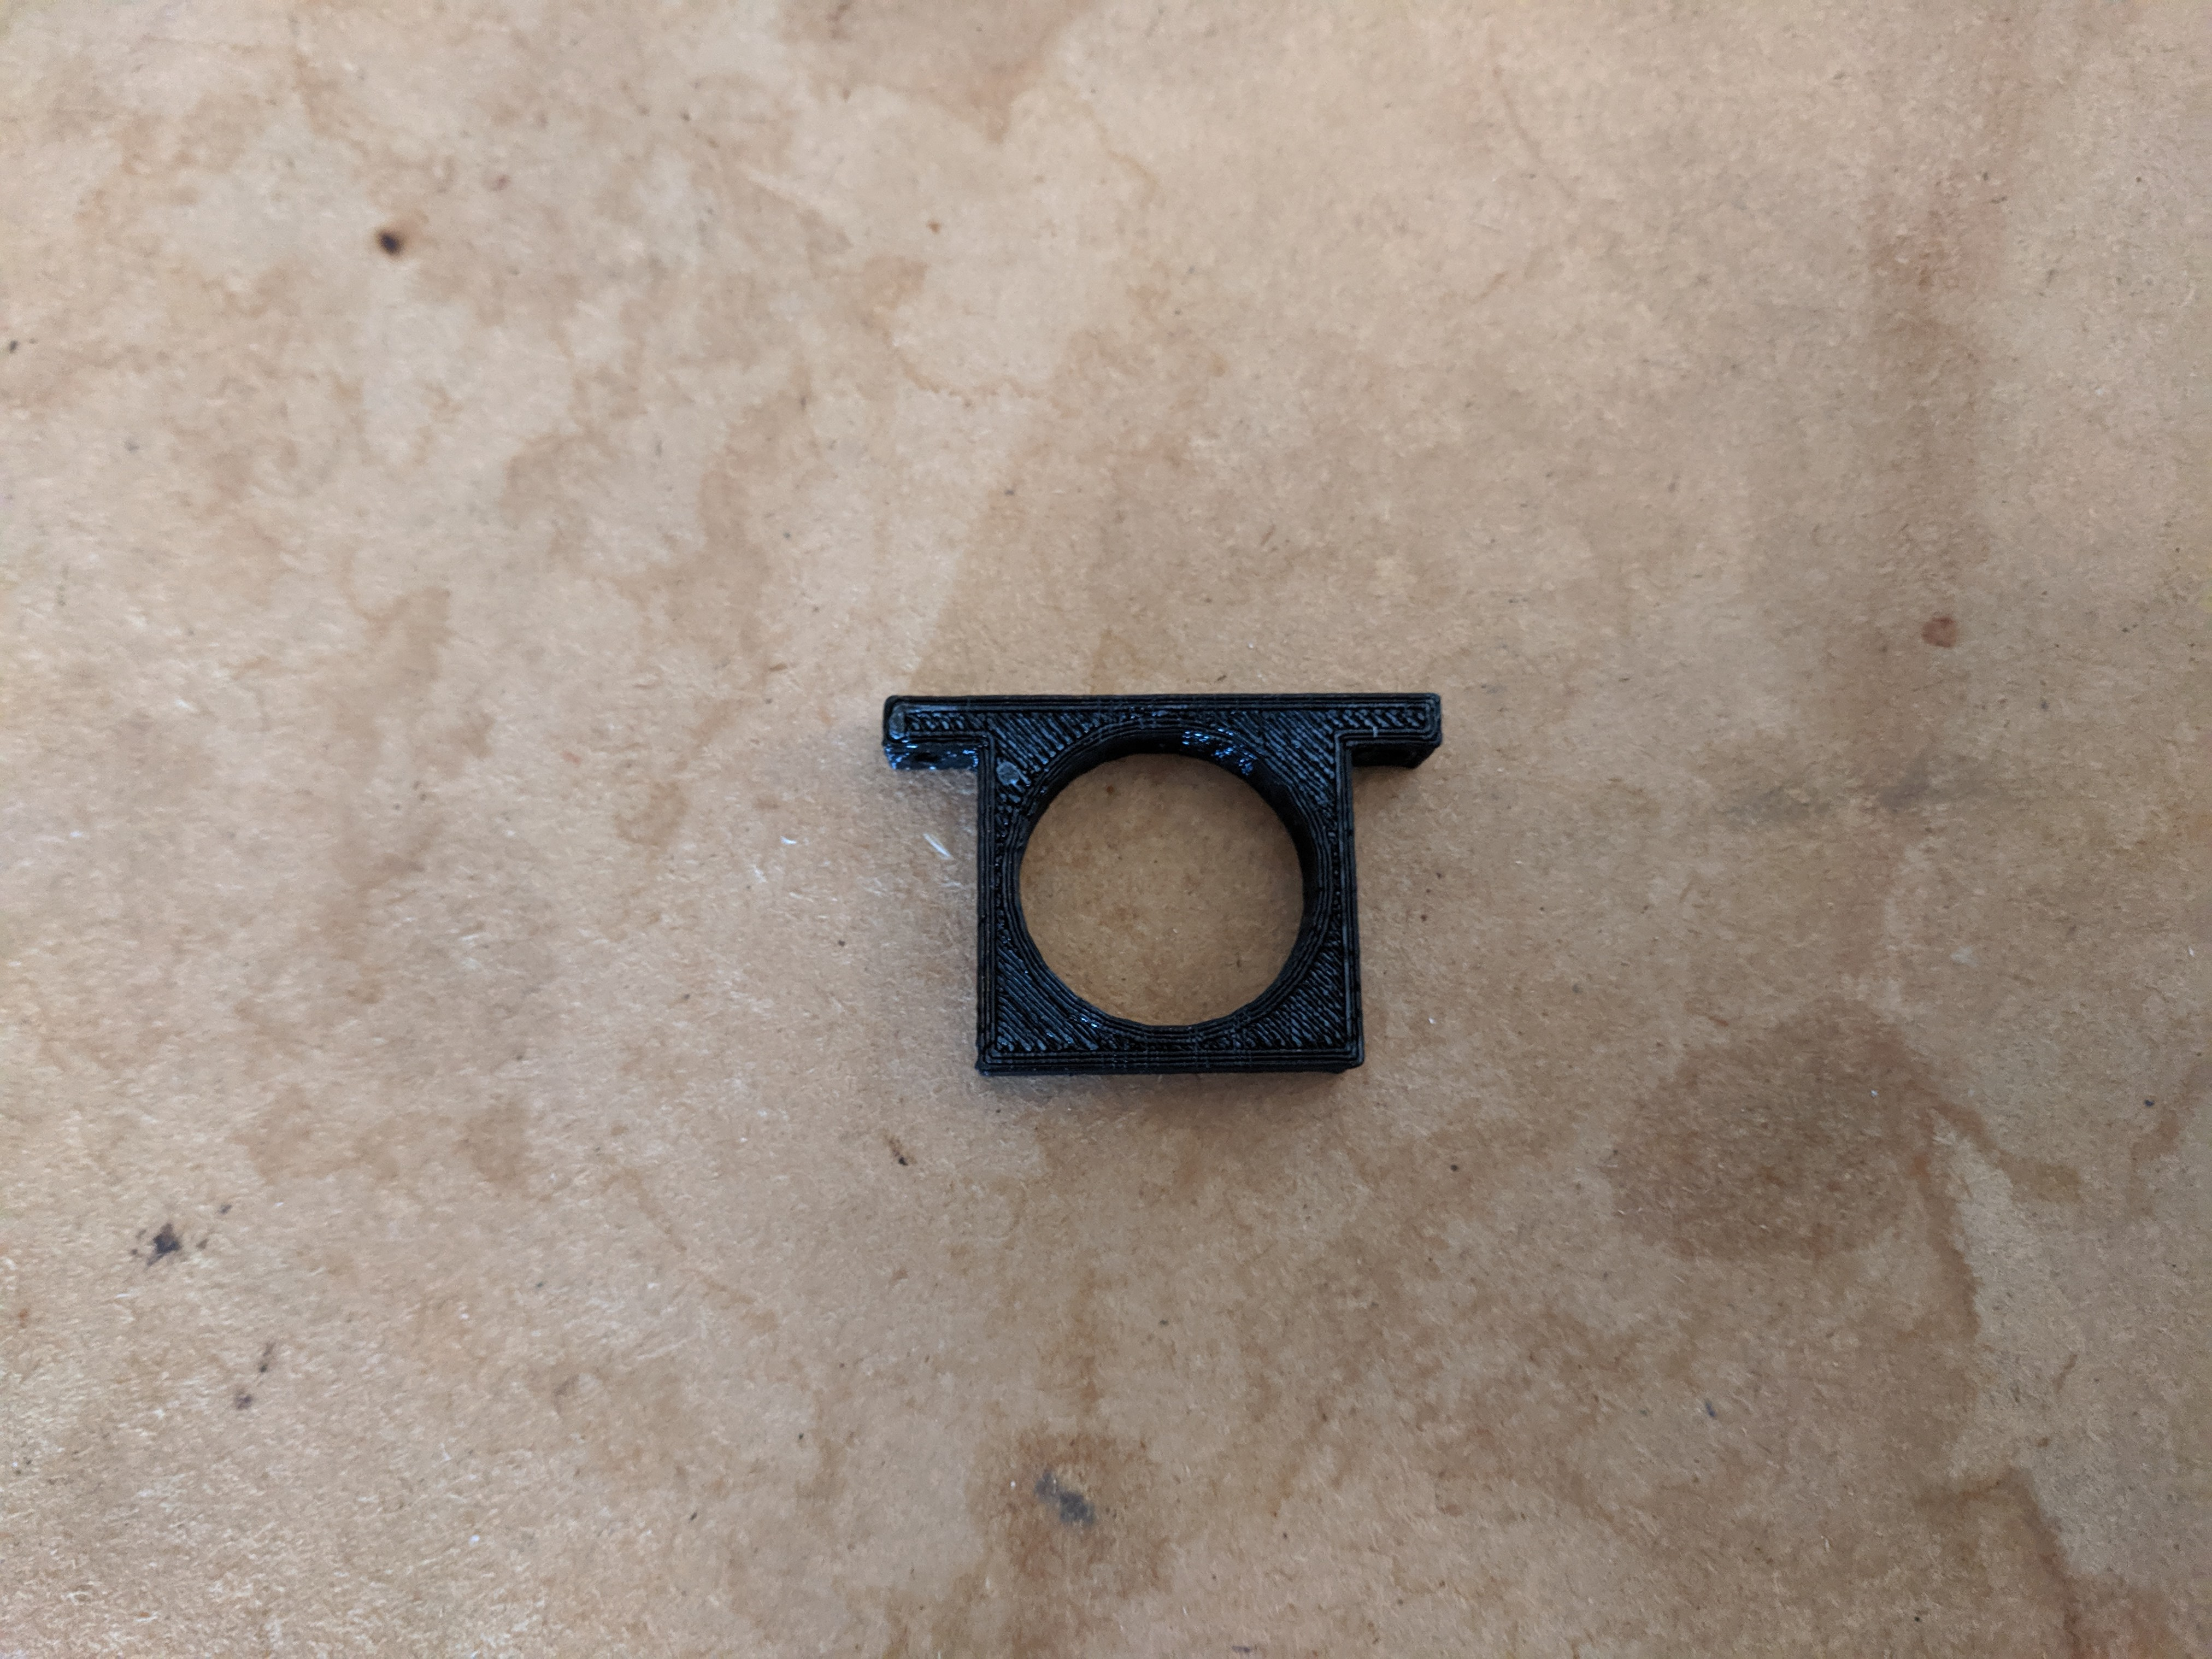
\includegraphics[height=5cm]{bearing_mount}}
		\caption{Plastic bearing mounts designed with Sketch up and constructed using additive manufacturing. Four of these were used.}
	\end{minipage}
	\hspace{1cm}
	\begin{minipage}[t]{0.45\textwidth}
		\centering
		
		\begin{tabular}{p{3.5cm}lr}
			\toprule
			Measurement & Value & Unit \\
			\midrule
			Diameter & 0.120 & $\si{\meter}$ \\
			Mass & 0.013 & $\si{\kilogram}$ \\
			 & & \\
			\bottomrule
		\end{tabular}
		
		\vspace{0.5cm}
		
		\frame{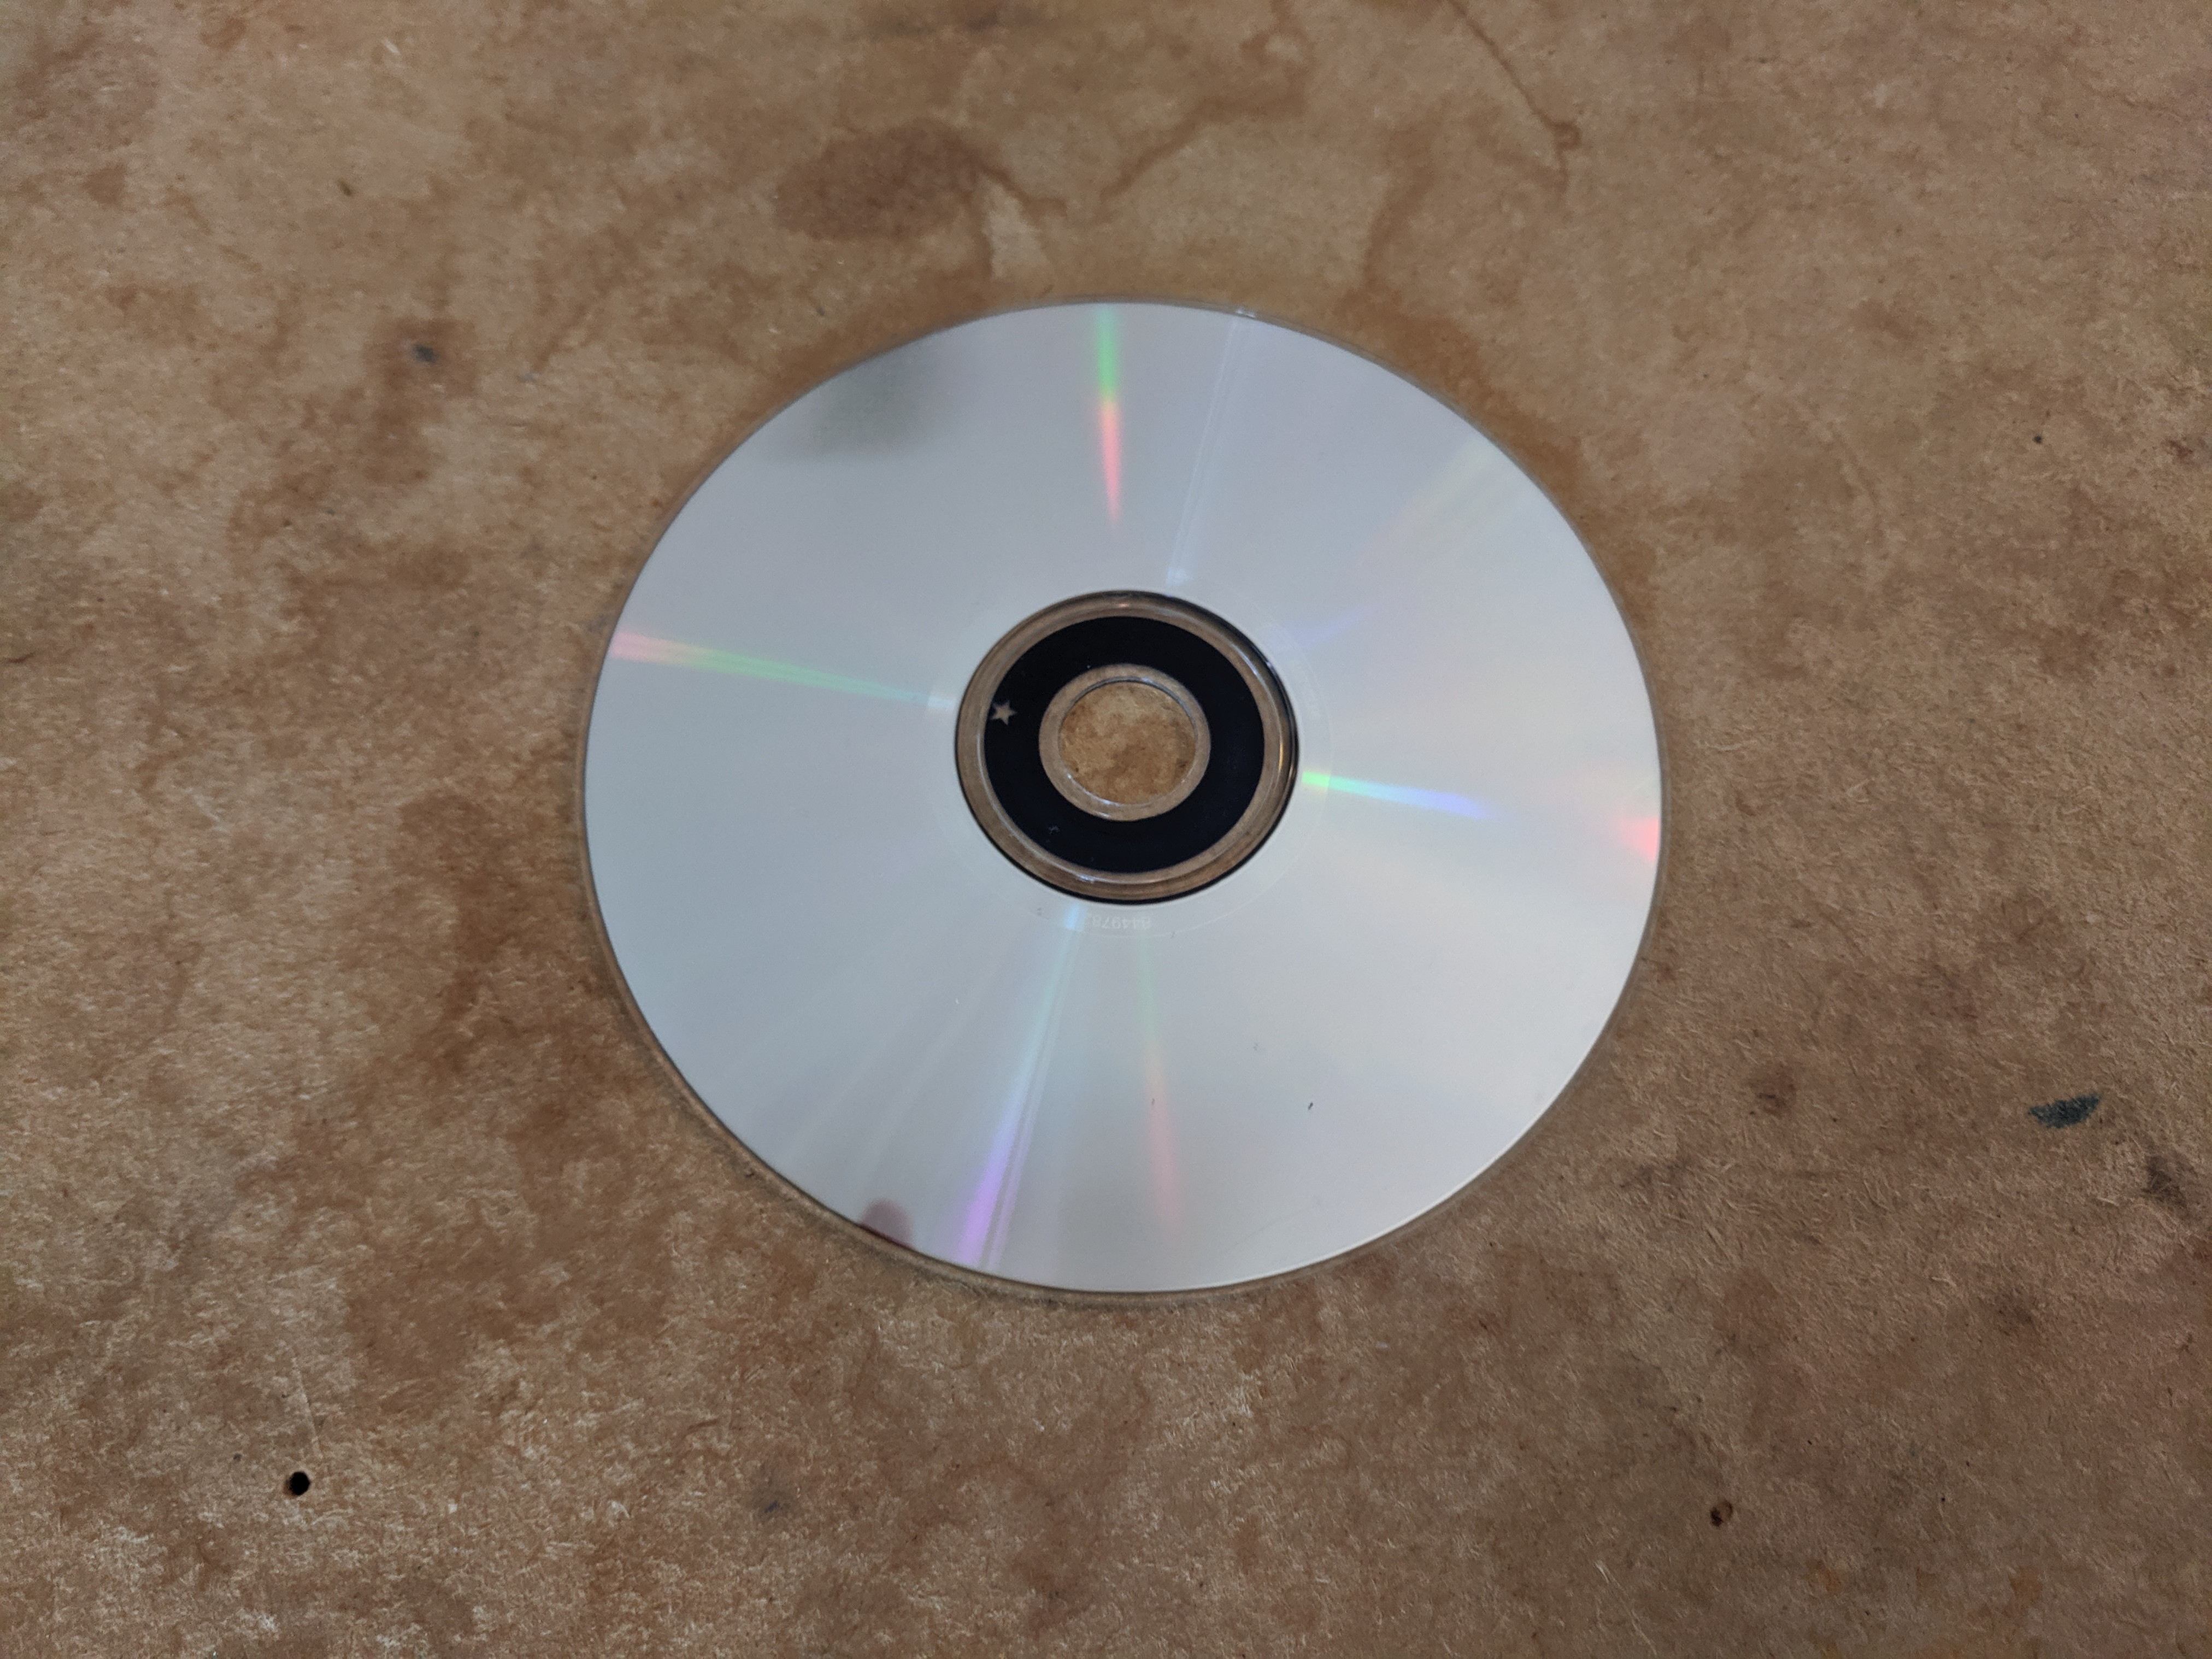
\includegraphics[height=5cm]{cd}}
		\caption{Compact disc used for wheels. Four of these were used.}
	\end{minipage}
\end{figure}


\begin{figure}[h]
	\centering
	\begin{minipage}[t]{0.45\textwidth}
		\centering
		\begin{tabular}{p{3.5cm}rc}
			\toprule
			Measurement & Value & Unit \\
			\midrule
			Length (Lever Arm) & 0.400 & $\si{\meter}$ \\
			Length (Shaft) & 0.100 & $\si{\meter}$ \\
			Mass (Lever Arm) & 0.011 & $\si{\si{\kilogram}}$ \\
			Mass (Lever Arm) & 0.003 & $\si{\si{\kilogram}}$ \\
			\bottomrule
		\end{tabular}
		
		\vspace{0.5cm}
		
		\frame{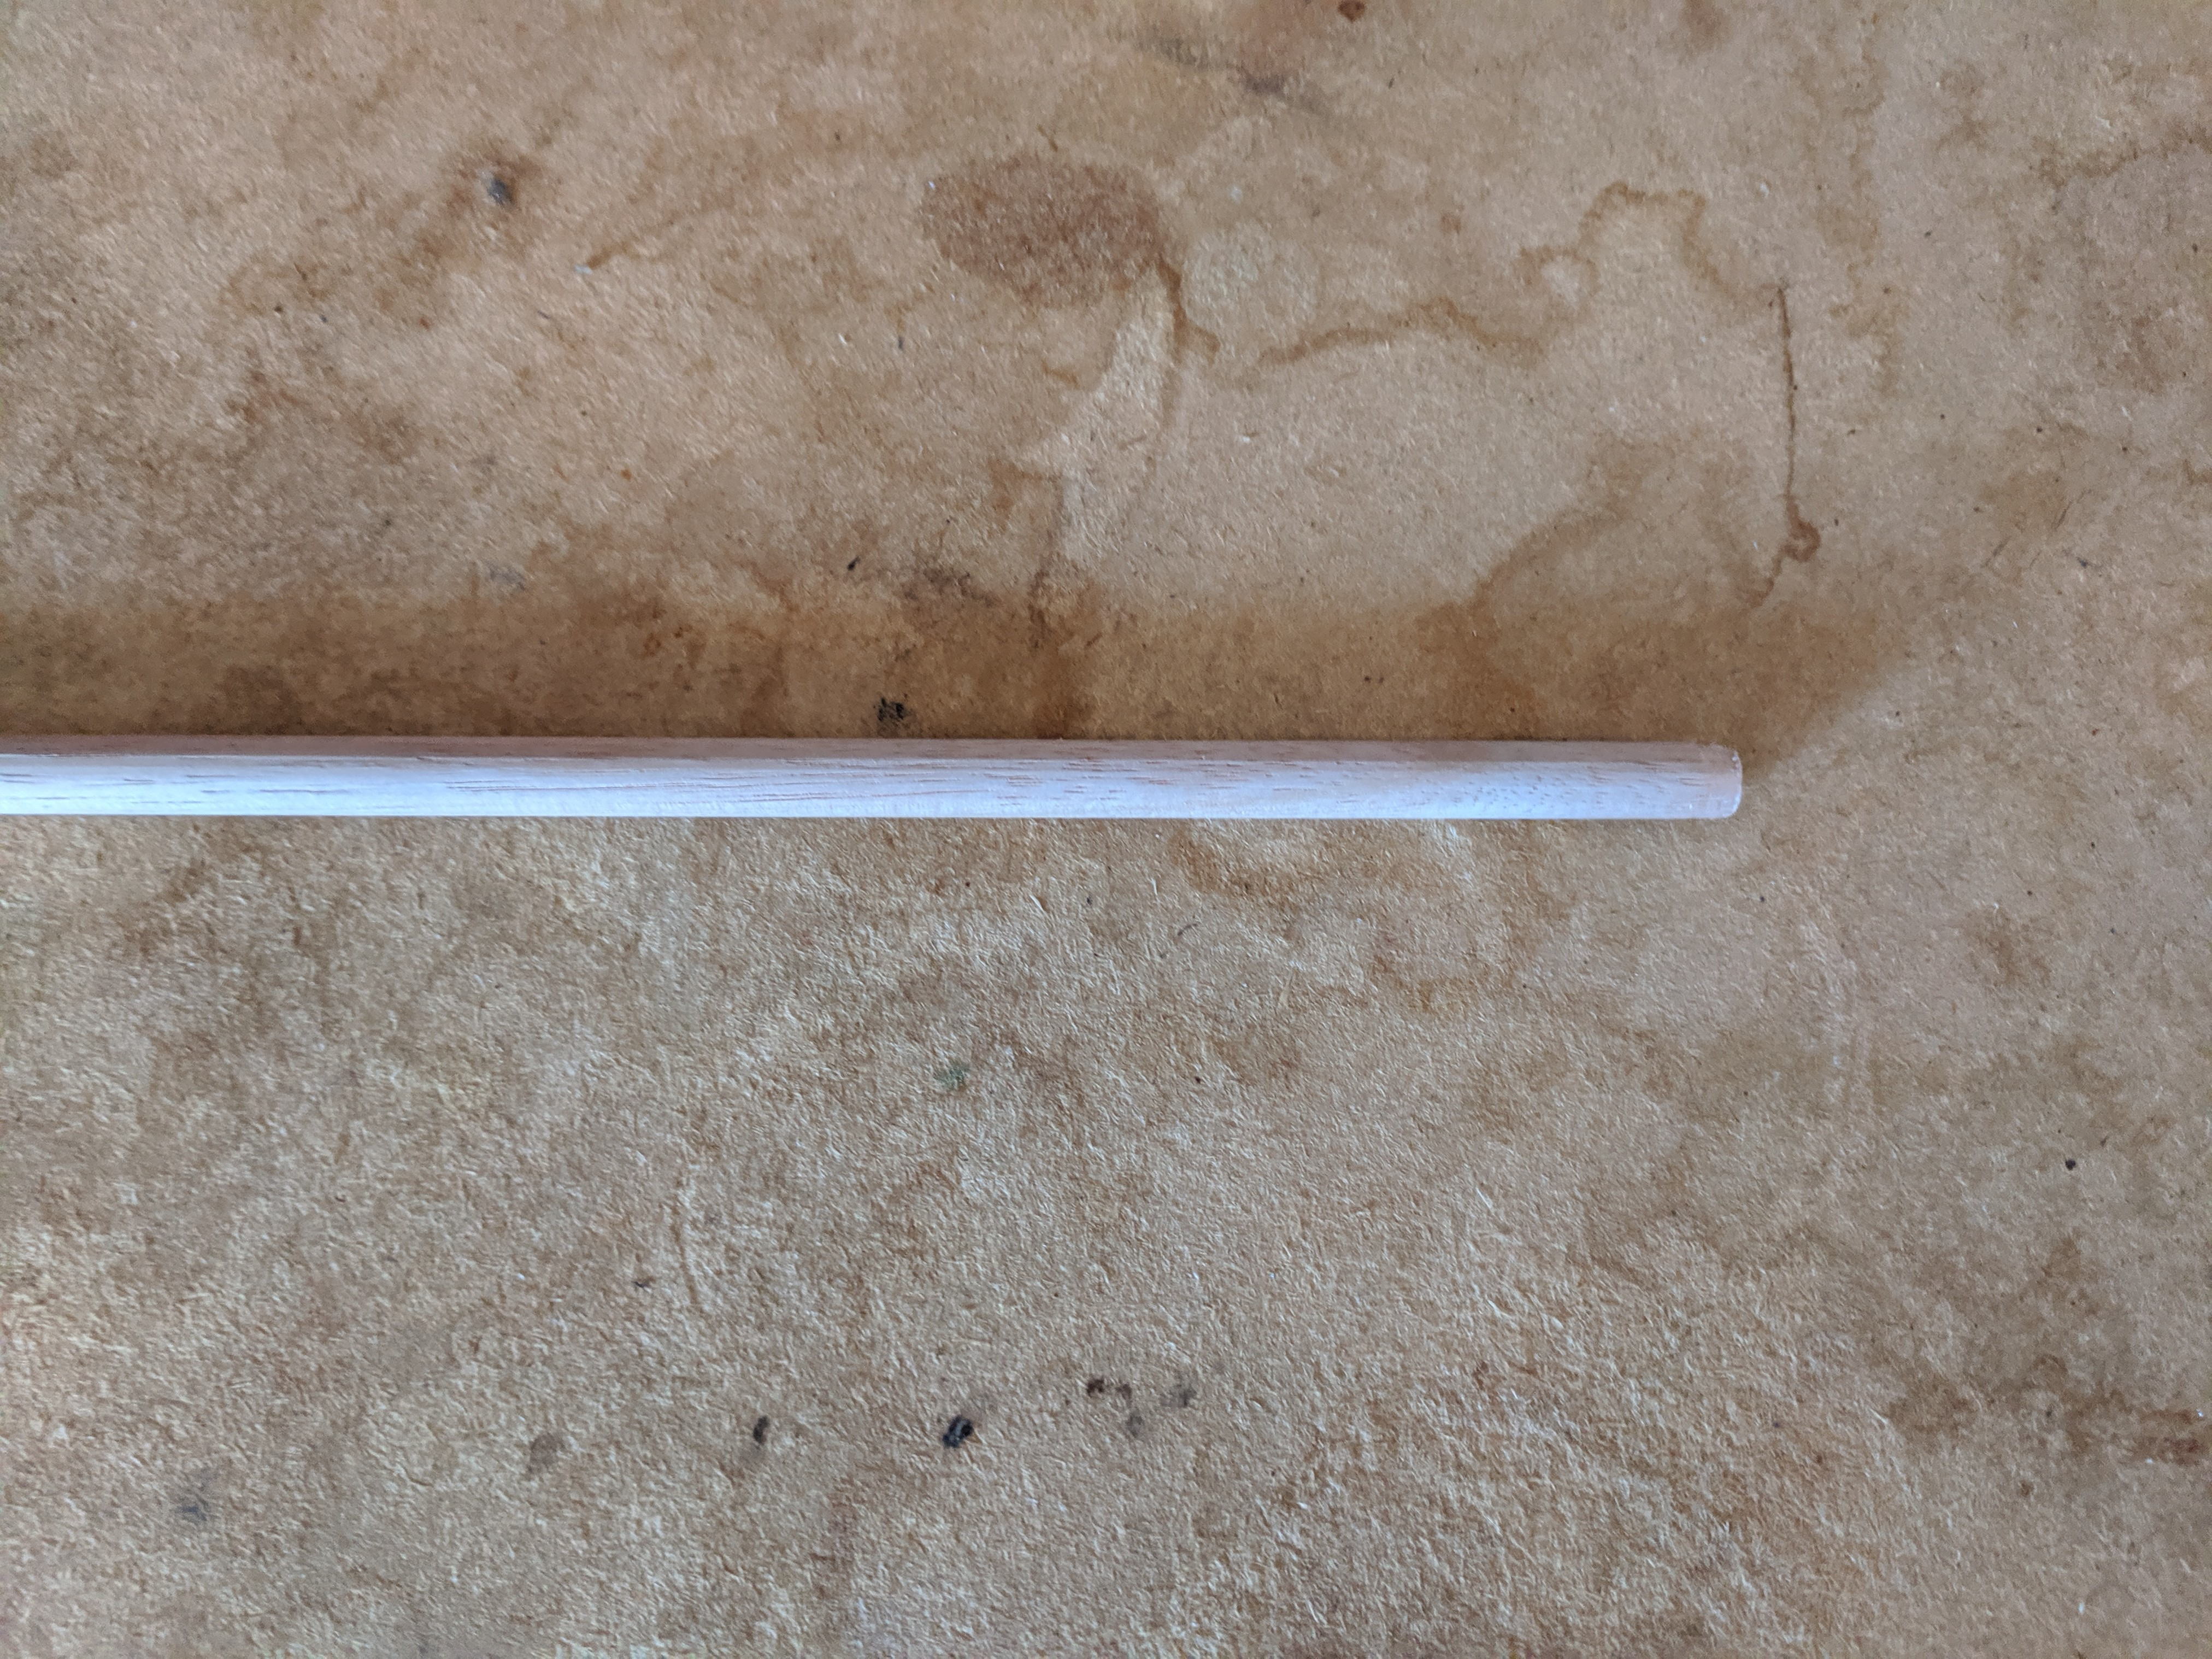
\includegraphics[height=5cm]{dowel}}
		\caption{Dowel lengths used for both the lever arm (one used), and for the shafts (two used) to which wheels were attached.}
	\end{minipage}
	\hspace{1cm}
	\begin{minipage}[t]{0.45\textwidth}
		\centering
		\begin{tabular}{p{3.5cm}rc}
			\toprule
			Measurement & Value & Unit \\
			\midrule
			Length & 0.100 & $\si{\meter}$ \\
			Width & 0.045 & $\si{\meter}$ \\
			Mass & 0.023 & $\si{\kilogram}$ \\
			 & & \\
			\bottomrule
		\end{tabular}
		
		\vspace{0.5cm}
		
		\frame{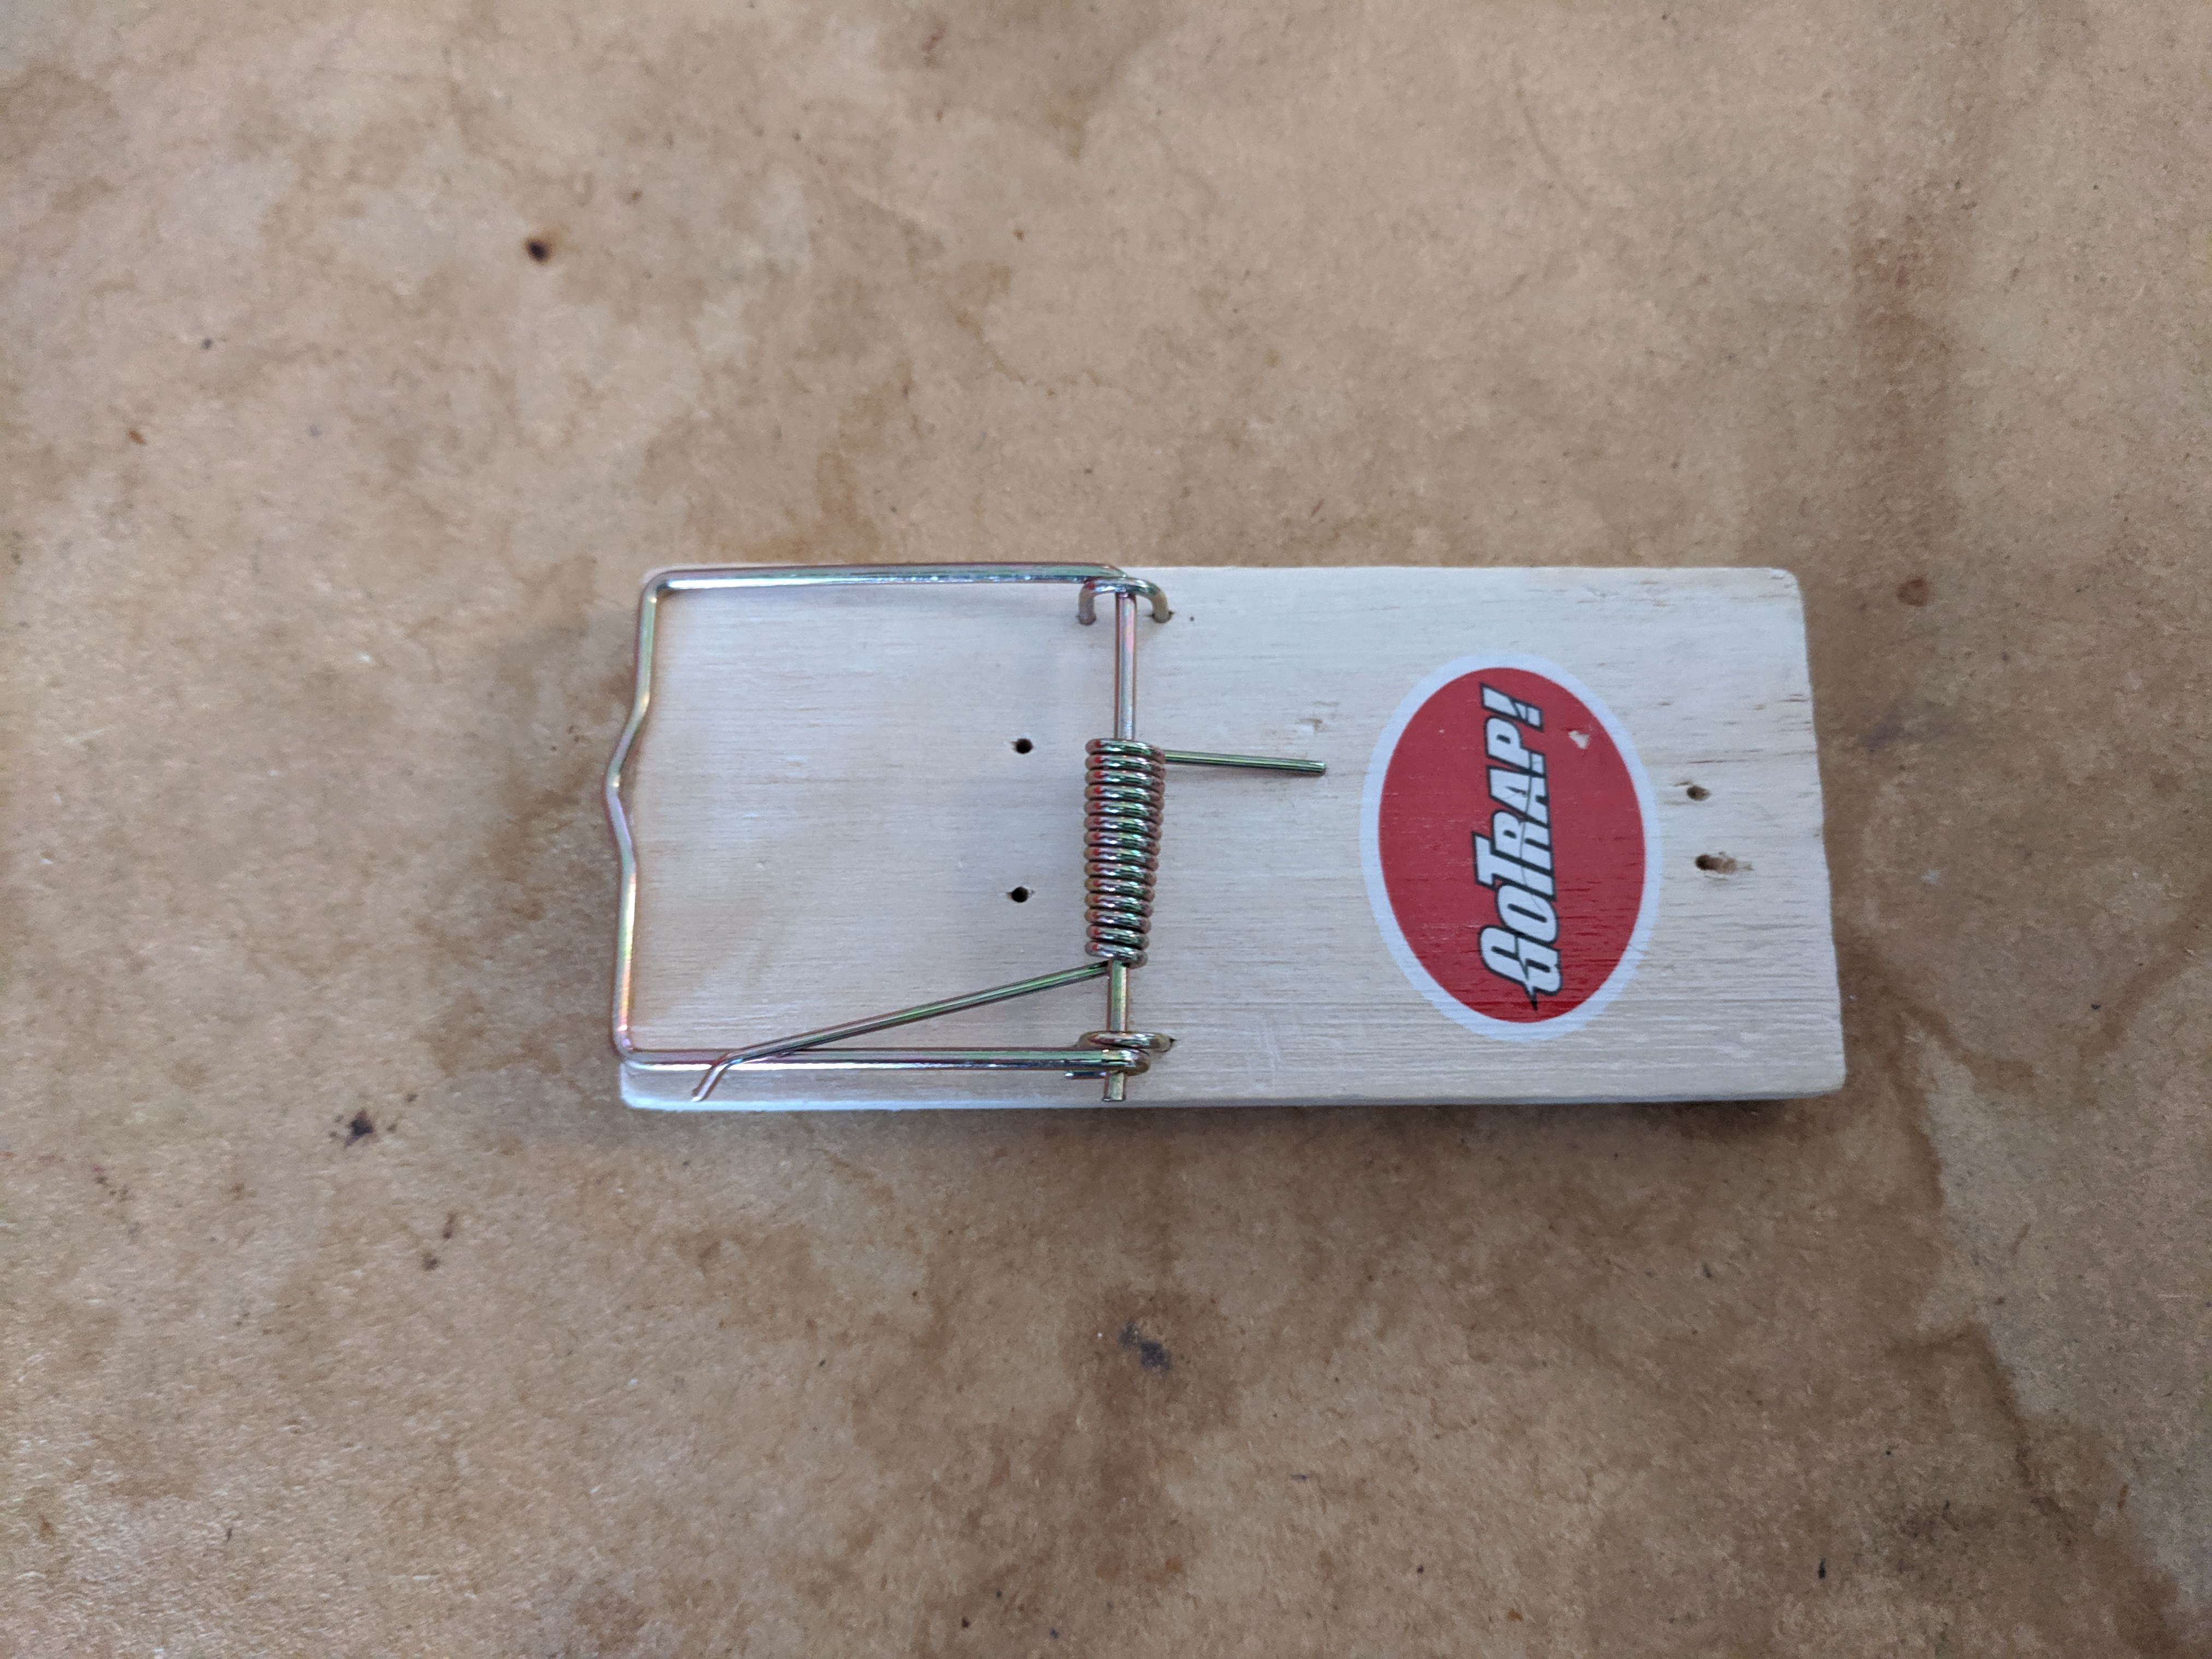
\includegraphics[height=5cm]{mouse_trap}}
		\caption{Mouse trap used to power vehicle.}
	\end{minipage}
\end{figure}

\clearpage

\section{Machine Dynamics}
\subsection{Theoretical Rolling Friction}

\subsection{Theoretical Static Friction}

\subsection{Theoretical Rotational Inertia of Wheels and Shaft}

\subsection{Spring Coefficient and Potential Energy}

\subsection{title}

\section{Distance Estimation}

\section{Experimental Performance and Possible Improvements}

\section{Conclusion}

\bibliography{my_bib}
\bibliographystyle{ieeetr}

\end{document}